
\section{Evaluation}
\label{sec:evaluation}

%In this section, we present a comprehensive evaluation of how well Inside-Out can predict end-to-end storage performance (latency, throughput and IOPS) 
%using low-level system metrics for a wide range of SDS environment.
In this section, we present a comprehensive evaluation of Inside-Out.
We demonstrate that Inside-Out can accurately predict end-to-end performance, 
i.e., throughput and IOPS, using low-level system metrics and
is applicable to a wide range of realistic scenarios.

%SDS offers wide flexibility for hosting storage services and in this section, we present comprehensive evalution to study whether low-level performance metrics can accurate end-to-end performance and Inside-Out can be applied for practical use in many SDS senarios.
%All SDS scenarios are listed in Table~\ref{tab:prediction_scenario}.


\subsection{Setup}
\label{sec:dataset}

%We choose Ceph as the storage service running on our SDS platform \cite{ceph}. 
%We use COSBench for measuring the storage performance \cite{cosbench}.
%COSBench supports several object storage protocols, including \textit{librados} used by Ceph. 
We choose Ceph~\cite{ceph} as a target distributed storage service for our evaluation and             
use COSBench~\cite{cosbench} to generate various types of storage workloads.
COSBench supports several object storage protocols, including \textit{librados} for Ceph, and
provides a set of knobs to change storage traffic pattern. 
Table~\ref{tab:cosbench_configurations} lists Ceph and COSBench configurations used in our experiments.
%We collected benchmarking data from three SDS clusters 
%located in a research lab of a major telecommunication company. 

\newcommand{\scenarioMU}{Increasing users}
\newcommand{\scenarioCUB}{Complex usage}
\newcommand{\scenarioCRB}{Complex request}
\newcommand{\scenarioWIB}{Write intensive}
\newcommand{\scenarioRIB}{Read intensive}
\newcommand{\scenarioMWIB}{Medium write intensive}
\newcommand{\scenarioMRIB}{Medium read intensive}
\newcommand{\scenarioMM}{Reconfigure Ceph}
\newcommand{\scenarioSUI}{Scale-up instances}
\newcommand{\scenarioMBS}{Medium network SLO}
\newcommand{\scenarioLBS}{Low network SLO}
\newcommand{\scenarioSON}{Scale out to}
\newcommand{\scenarioSIN}{Shrink in to}
\newcommand{\scenarioMTA}{Case 1 - tenant 1 (250 Mbit)}
\newcommand{\scenarioMTB}{Case 1 - tenant 2}
\newcommand{\scenarioMTAA}{Case 2 - tenant 1}
\newcommand{\scenarioMTBB}{Case 2 - tenant 2}


\newcommand{\spheading}[2][10em]{% \spheading[<width>]{<stuff>}
  \rotatebox{90}{\parbox{#1}{\raggedright #2}}}

\begin{table*}[t!]
  \fontsize{8}{8}\selectfont
  \centering
  \caption{Common scenarios that storage behavior can change in a software-define storage environment}
  \begin{tabularx}{.95\linewidth}{|l|c|c|c|X|}
  \hline
  & \textbf{Scenario} & \textbf{Training Dataset} &  \textbf{Prediction Dataset} & \textbf{Explanation} \\
  \hline
  \multirow{7}{*}[-0.3ex]{\rotatebox[origin=c]{90}{\textbf{Changing Workload}}} & \scenarioMU & \{1, 2\} & \{4\} & The number of client virtual machines running COSBench. \\
  \cline{2-5}
  & \scenarioCUB & \{1, 2, 4, 8\} & \{16, 32\} & The number of threads for all benchmark clients. \\
  \cline{2-5}
  & \scenarioCRB & 512KB & 1-1024KB & The request size (either static or variable) of the workload, configured in COSBench. \\
  \cline{2-5}
  & \scenarioWIB & \{50, 75, 100\} & \{25, 0\} & \multirow{4}{1\linewidth}{The percentage of read operations the workload. The read and write percentages are 100 in total.}\\
  \cline{2-4}
  & \scenarioRIB & \{0, 25, 50\} & \{75, 100\} & \\
  \cline{2-4}
  & \scenarioMWIB & \{0, 50, 100\} & \{25\} & \\
  \cline{2-4}
  & \scenarioMRIB & \{0, 50, 100\} & \{75\} & \\
  \hline
  \hline
  \multirow{4}{*}[-1.7ex]{\rotatebox[origin=c]{90}{{\textbf{Reconfiguration}}}} & \scenarioMM & \{1\} & \{2\} & The number of Ceph monitor daemons.\\
  \cline{2-5}
  & \scenarioSUI & m1.small & m1.medium & The instance type of the virtual machines running Ceph is upgraded to a powerful one.  A m1.small instance has one core and 2GB memory and m1.medium has two cores and 4GB memory.  Note that in this setting, the configuration of disk I/O remains the same.\\
  \cline{2-5}
  & \scenarioMBS & unrestricted & 500 Mbps & The network bandwidth of virtual machines is limited at 500 Mbps.  We use the Linux tool \textit{tc} for network throttling\\
  \cline{2-5}
  & \scenarioLBS & unrestricted & 250 Mbps & Network bandwidth is limited at 250 Mbps.\\
  \hline
  \hline
  \multirow{2}{*}[-0.5ex]{\rotatebox[origin=c]{90}{\textbf{Elasticity}}} & \scenarioSON { \textit{n}} & \{4, 6, 8, 10\} & \{20, 30, 40\} & The total number of Ceph OSDs.  Note that each OSD is running in a virtual machine and different OSDs can run on the same physical servers (10 servers in total). \\
  \cline{2-5}
  & \scenarioSIN { \textit{n}} & \{20, 30, 40\} & \{4, 6, 8, 10\} & Similar to the above, but the cluster size is decreased. \\
  \hline
  \end{tabularx}
  \label{tab:prediction_scenario}
\end{table*}

\begin{table}[htp]
 \centering
 \caption{Ceph and COSBench settings for data collection.}
 \begin{tabular}{ ll  }
  \hline
  \textbf{\normalsize{Parameters}} & \textbf{\normalsize{Values}} \\
  \hline
  \textbf{Ceph version} & 9.2 (Infernalis) \\
  \textbf{\# of physical nodes} & 16 \\
  \textbf{Storage back end} & Logic Volume (iSCSI) \\
  \textbf{\# of storage nodes} & \{4, 6, 8, 10, 20, 30, 40\}\\
  \textbf{\# of drivers} & \{1, 2, 4\} \\
  \textbf{\# of workers} & \{1, 2, 4, 8\} \\
  \textbf{Request size} & \{512KB, 1-1024KB\} \\
  \textbf{Duration} & 180 sec \\
  \textbf{\# of containers} & \{64\} \\
  \textbf{\# of objects} & \{1024\} \\
  \textbf{read/write ratio} & \{100/0, 75/25, 50/50, 25/75, 0/100\} \\
  \hline
 \end{tabular}
 \label{tab:cosbench_configurations}
\end{table}



We collected benchmarking data from an OpenStack-based SDS platform.
The cluster has 16 machines, and
each machine has 16 cores, 24GB memory and 250GB disk space.
Each machine has 1Gbps network interface connected to a 10Gbps switch.
The dataset is collected from about 5300 benchmark runs. The total dataset is composed of about 15.2 million records, each of which is 
a vector of 32 low-level performance data.
The end-to-end performance data collected from COSBench contains 
3 million records. 
The combined dataset is about 24GB, collected over two weeks. 

%[comment: please briefly describe cluster A/B/C in text as well (using the table II's content). we need to be kind.]
%The dataset is collected from 8300 benchmark runs in total; 5300 runs on \textit{Cluster A}, 
%1500 runs on \textit{Cluster B}, and 1500 runs on \textit{Cluster C}.
%The total number of records of low-level performance data is more than 18 million 
%and each record is a vector with 32 metrics.
%Our resulting dataset is made up of 18 million records, each of which is 
%a vector of 32 low-level performance data.}
%The number of records for \chin{end-to-end} performance data collected from COSBench contains 
%\chin{3.6 million} records, which is one-fifth of the low-level records.
%The combined dataset is about 34GB, and is worth about two-week measurements in total.
%All raw performance data can be found at \chin{http://xxx.xxx}.
%RP: We cannot publish any data without approval from AT&T.


\subsection{The Comparison Method}
Our goal is to find a function $f(X_t)$ that predicts the end-to-end performance, where $X_t$ is a vector that describes the internal status at time $t$ of a distributed storage service.
We say a model is accurate if $f(X_t)=\hat{y_t} \simeq y_t$, where $y_t$ is the ground truth (measured at the client side) and $\hat{y_t}$ is the predicted values.
To interpret performance models, we are interested in four indicators:
1) the overall prediction accuracy,
2) the goodness-of-fit,
3) the consistency across diverse scenarios and
4) the consistency across prediction instances.

First, we use mean absolute percentage error (MAPE) to compute prediction accuracy as 
\setlength{\abovedisplayskip}{0pt} \setlength{\abovedisplayshortskip}{0pt}
%\begin{center}
\begin{equation} \label{eq:prediction_accuracy}
max(1 - \frac{\sum_{t=1}^{n} {|\frac{y_t - \hat{y_t}}{y_t}|}}{n}, 0)
\end{equation}
%\end{center}
where $n$ is the length of the observation period.
%For example, for a three-minute measurement period with one-minute sampling window, 
%if the measured performance values are $[10, 20, 30]$ and the predicted values are $[9, 18, 33]$, the average prediction accuracy is $90\%$.
We restrict the scope of prediction accuracy between $0$ to $1$ because the prediction accuracy can be negative (e.g. when $y_t$ is small).

Second, we use the coefficient of determination $R^2$ to interpret \emph{Goodness-of-Fit}, which is less than or equal to one \cite{Noorshams2013}.
Third, we examine whether a performance model can present consistent prediction in various SDS scenarios.
Last, we further analyze the probability density function of prediction decisions for different categories of prediction scenarios.

We consider prediction of throughput and IOPS for both read and write operations, and use the following terms $TP_r$, $TP_w$, $OP_r$ and $OP_w$ for read 
throughput, write throughput, read IOPS and write IOPS, respectively.



\subsection{Baseline: Prediction Performance on Static Deployment}
%

We evaluate prediction accuracy of Inside-Out under a variety of scenarios 
with different storage workloads and configurations
listed in Table~\ref{tab:prediction_scenario}.
In this subsection, we focus on a static deployment scenario with one storage tenant 
running on a distributed Ceph storage service that does not expand or shrink in terms 
of number of VMs used for running Ceph.
Later, we evaluate more challenging scenarios 
in which the Ceph cluster expands or shrinks based on user demand,
and storage traffic of multiple tenants interfere with each other.

%with the Ceph cluster expanding or shrinking based on user demand, 
%and multiple tenants interfering with each others storage traffic. 
%shows various scenarios where the prediction dataset differs from the training dataset.



\vspace{1ex}
%\subsection{Changing Workload}
\subsubsection{Can Inside-Out handle diverse workloads?}
\label{sec:changing_workload}

\begin{figure}
    \centering
    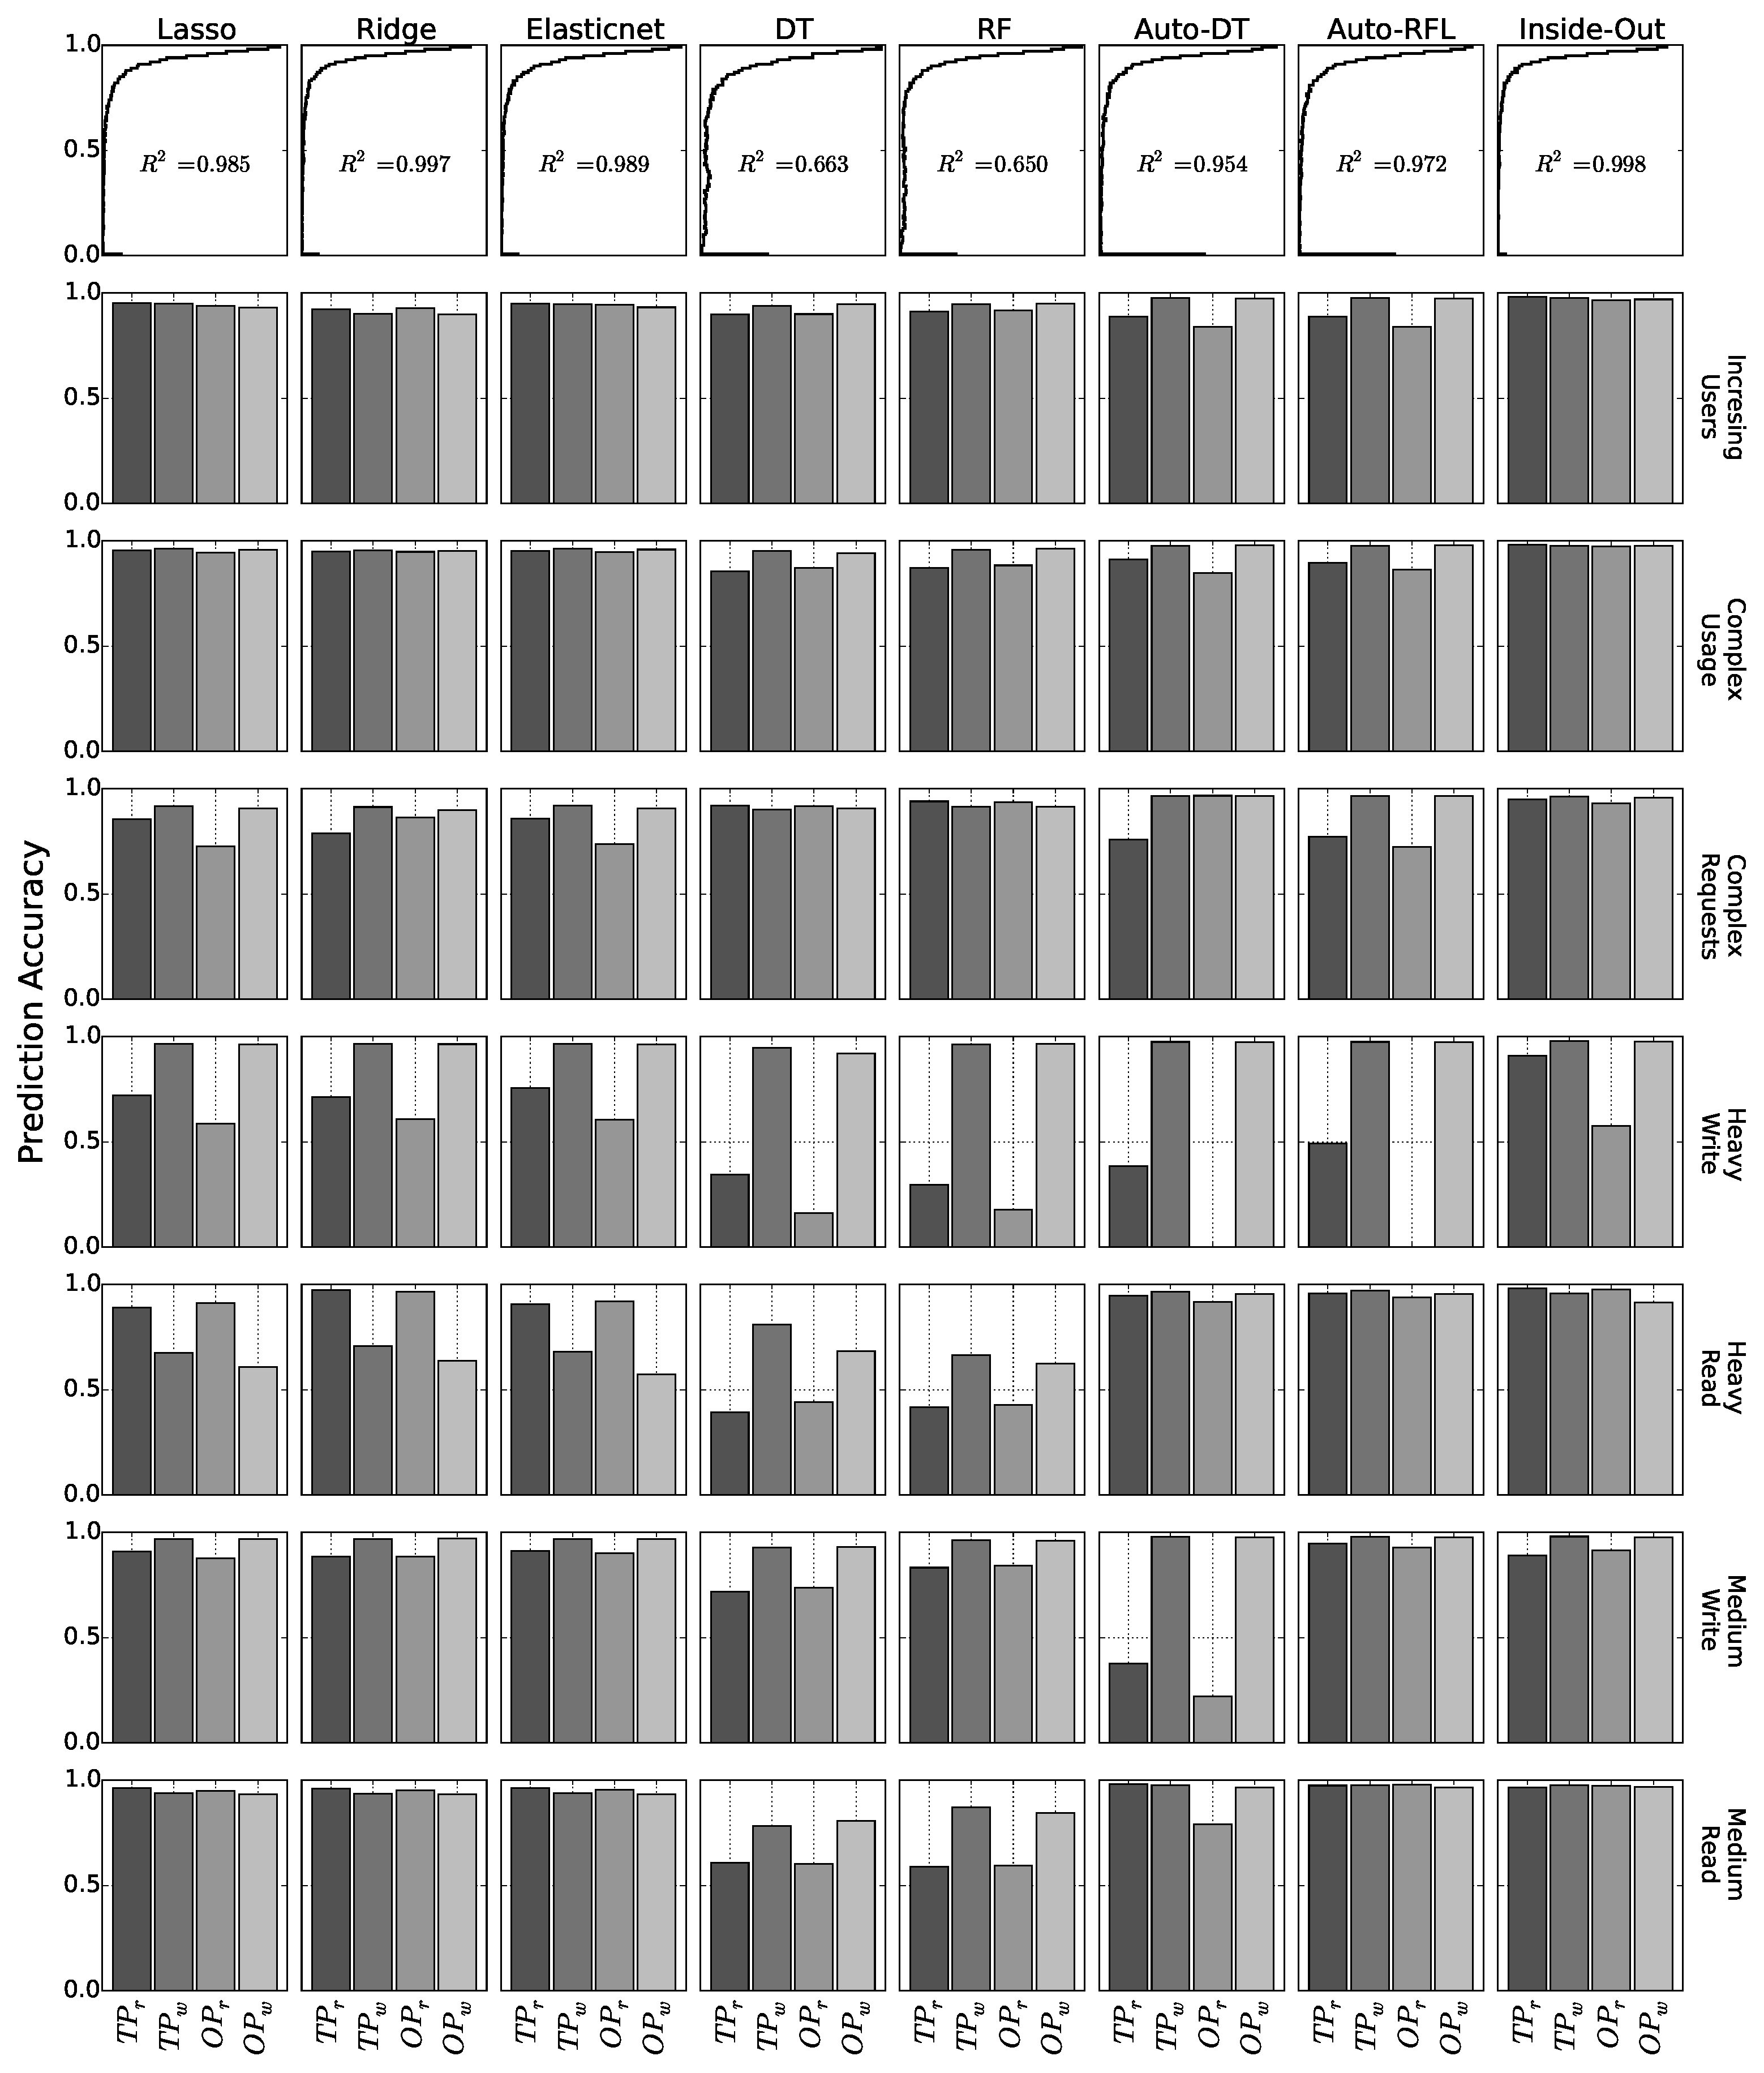
\includegraphics[width=0.9\textwidth]{Chapter-InsideOut/figures/unseen_workload_all_new.eps}
    \caption{Analysis of performance models with diverse workloads. Each bar is the average prediction accuracy. The top row is the probability density function of prediction accuracy for each performance model.}
    \label{fig:changing_workload}
\end{figure}

%\hfill\break

An SDS application needs to handle various request volumes, object/file sizes and different ratios of read/write workloads.
%In practice, it is difficult to obtain a training dataset that includes all access patterns.
First we examine whether Inside-Out can achieve accurate and consistent predictions when workload changes.


\paragraph*{Changing user behavior}
%\textbf{Changing user behavior.}

We increase the number of concurrent clients to stress the Ceph cluster.
%We push the Ceph cluster to a certain limit by increasing the parallelism of clients.
The \emph{\MakeLowercase{\scenarioMU}} scenario changes the number of COSBench clients and the \emph{\MakeLowercase{\scenarioCUB}} scenario increases the worker threads of each client.
As shown in \myfigure{\ref{fig:changing_workload}}, all prediction models perform well. The linear regression technique performs slightly better than the tree-based learning.
The linearly increasing load is well captured by linear models because of proportional change in low-level metrics.
When we switch to the \emph{\MakeLowercase{\scenarioCRB}} scenario, the variable request size slightly changes the behavior of Ceph, affecting prefetching and caching. 
We observe that the linear regression methods (Lasso, Ridge and Elastic Net) show drops in accuracy, e.g. 20\% in the $OP_r$ case; however, Inside-Out 
maintains good accuracy. 
The tree-based learning shows comparable predictions (5-10\% lower) with Inside-Out in these settings.



%\textbf{Complex request behavior.}
%Next, we change the workload from a constant IO request size to variable size.
%In this case, Inside-Out slightly improves the prediction accuracy over Lasso, %and outperforms the three linear models.
%Auto-DT and Auto-RFL show inconsistent prediction result with about 15\% %degradation of accuracy, comparing with the best case.
%One possible expalantion is that some important features filtered by DT and RF 
%are removed.
%Lasso and Elastic Net encounters accuracy drop in the read IOPS prediction


\paragraph*{Varying I/O pattern}

%The workload is a strong performance factor to a storage system \cite{Noorshams2013}.
%The read performance, for example, is affected by the amount of concurrent read or write operations.
Next, we consider workloads with different ratios of read to write operations.
\myfigure{\ref{fig:changing_workload}} shows that varying workload poses a big challenge to performance models. 
The linear regression methods (Lasso, Ridge and Elastic Net) present better prediction accuracy than tree-based models (DT, RL).
In addition, we observe that several models make poor predictions of $TP_r$ and $TP_r$.
The reason is that read behavior is largely affected by \textit{cache}, and large read variance contributes to low prediction accuracy.
Inside-Out performs consistently well, whereas the three linear regression techniques show accuracy drops.
One exception is the $OP_r$ prediction in the \textit{write-intensive} scenario even though $TP_r$ prediction is accurate.
As we will show later in Section~\ref{sec:online_learning}, \emph{over- and under-predictions} cause such behavior. 
The self-learning property of Inside-Out improves its prediction accuracy as it keeps learning the new storage behavior.


\begin{figure}
    \centering
    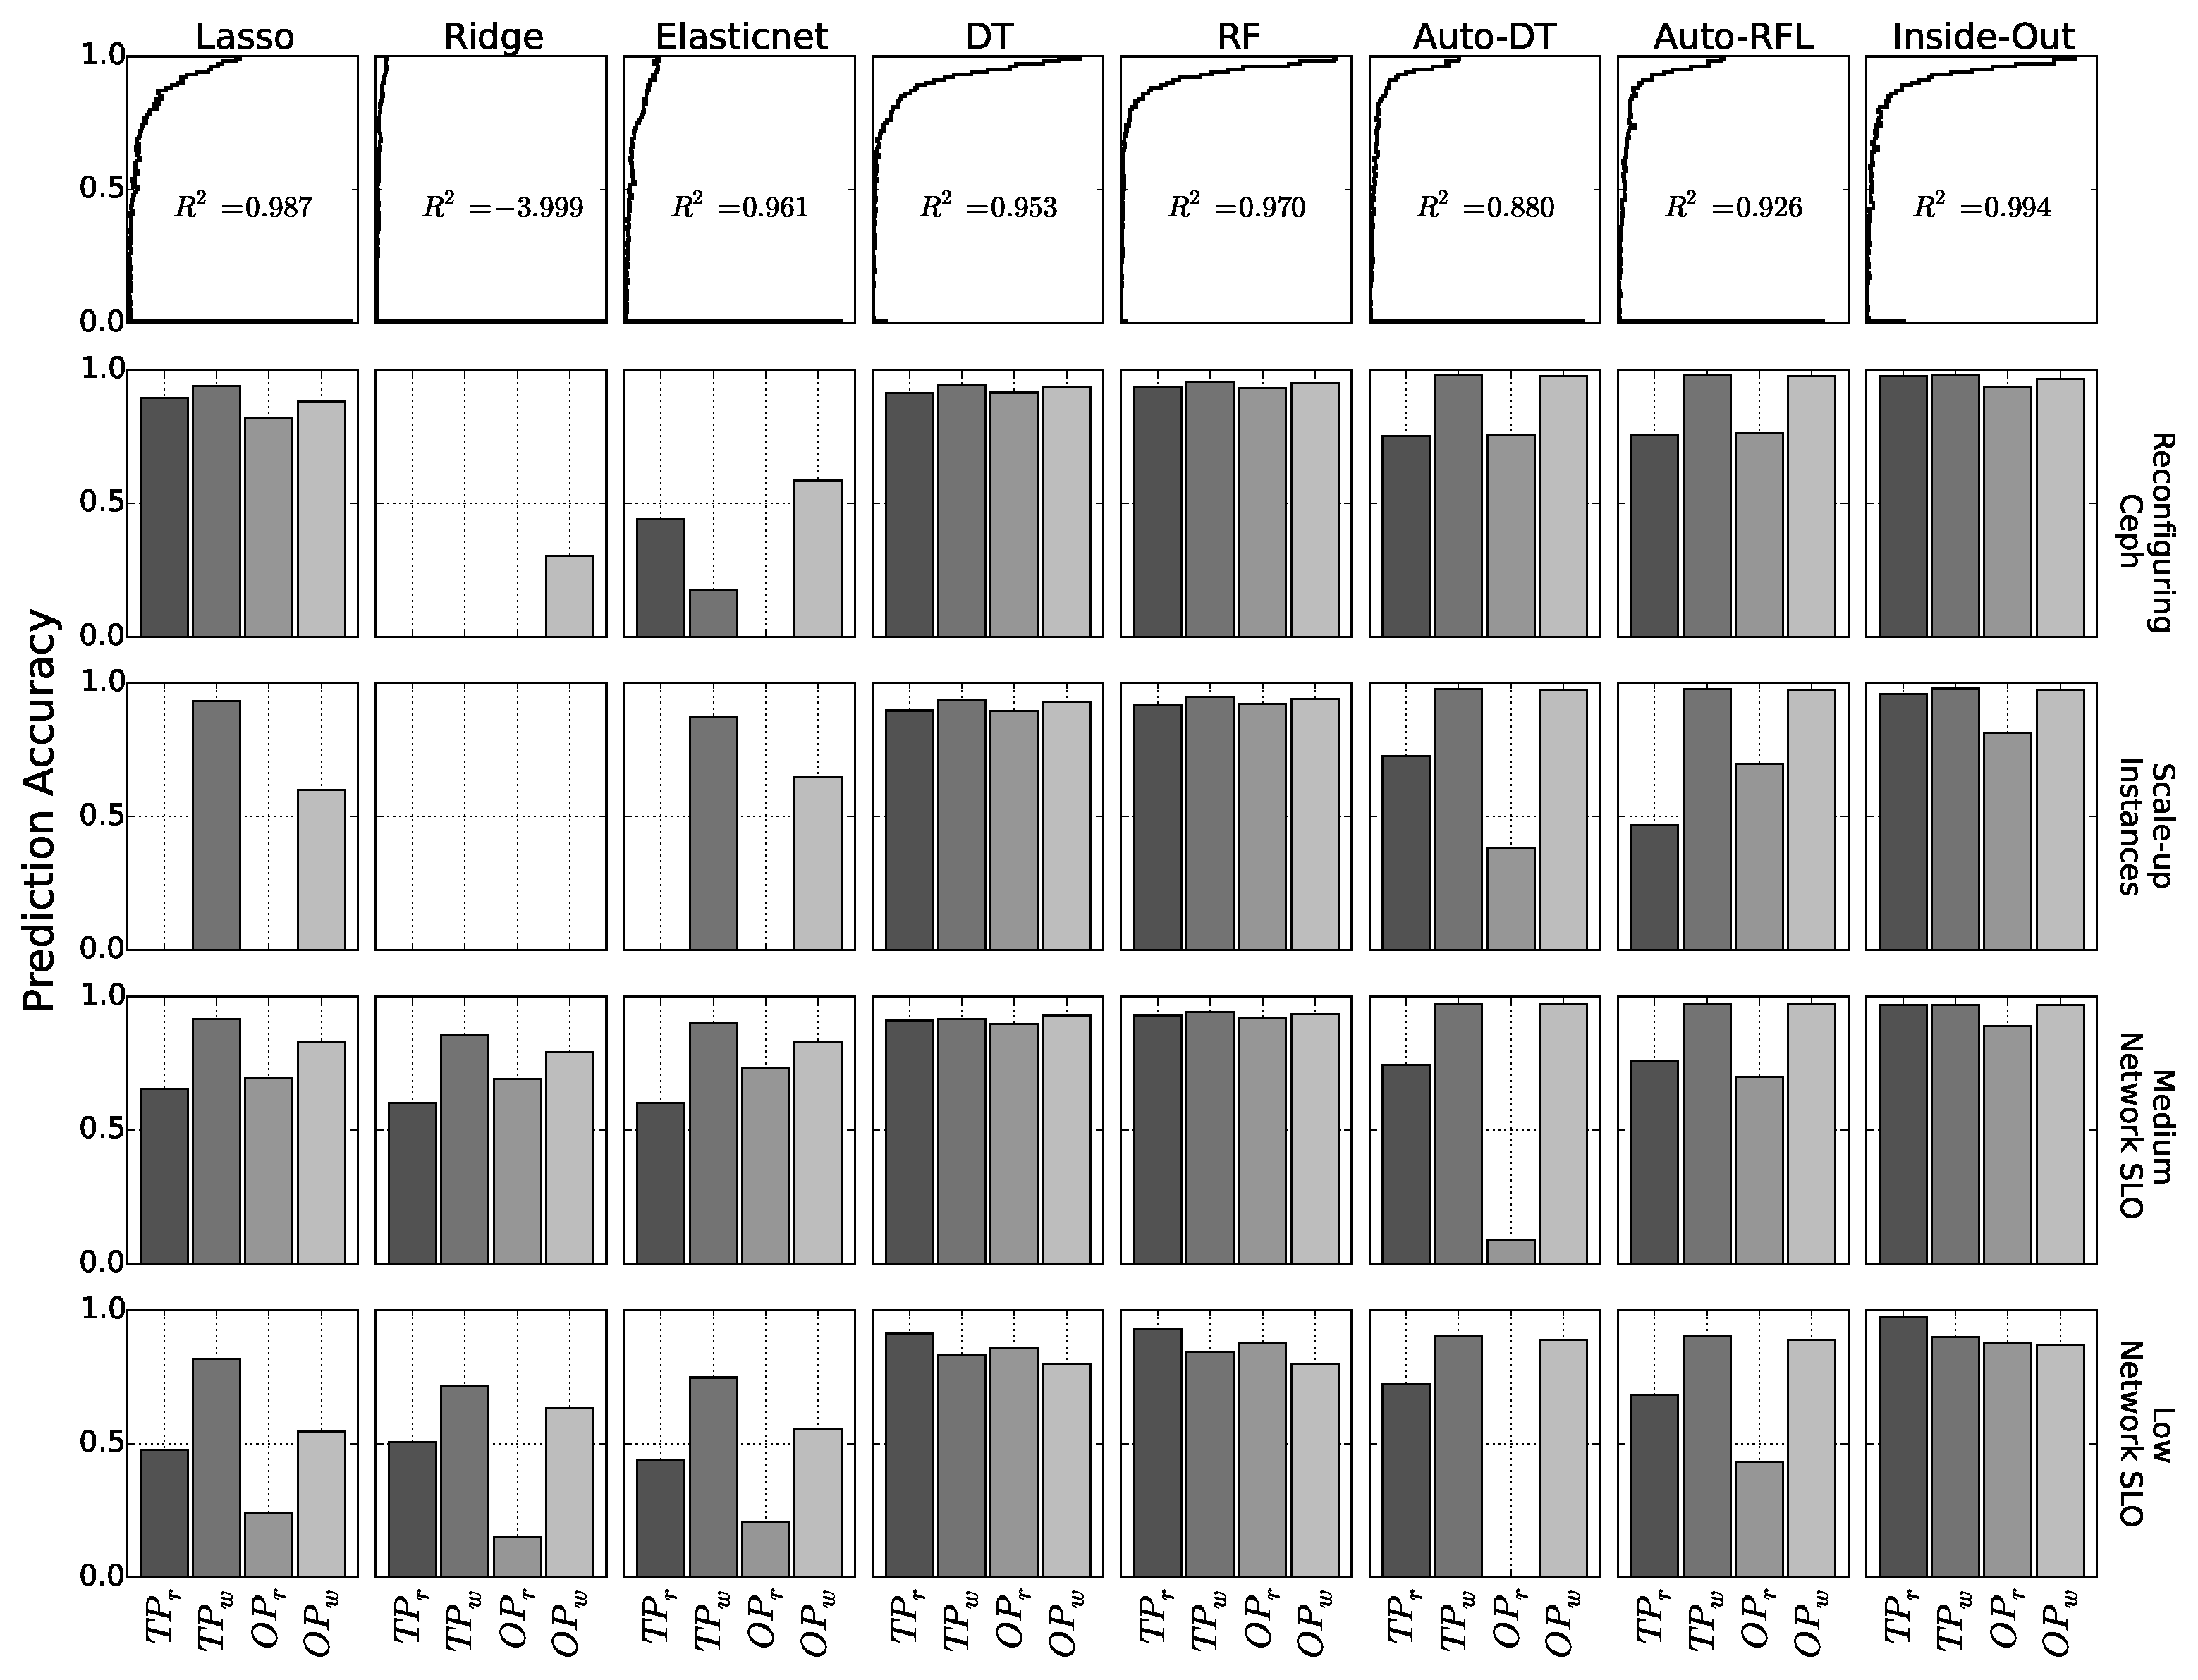
\includegraphics[width=0.9\textwidth]{Chapter-InsideOut/figures/unseen_configuration_all_new.eps}
    \caption{Comparison of performance models when the storage service is reconfigured: Ceph, VMs and network SLOs}
    \label{fig:reconfiguring_storage}
\end{figure}


\paragraph*{Summary}
The linear regression models achieve high prediction accuracy, great goodness-of-fit ($>0.98$) and consistency in prediction 
for many instances (see the distribution of prediction accuracy in \myfigure{\ref{fig:changing_workload}}), but they 
are not consistent across all prediction scenarios.
Inside-Out achieves good prediction accuracy across all cases consistently because the two-level approach 
filters out many irrelevant features in the first step, thereby presenting a smaller relevant feature space to the second step. 
The tree-based learning methods (DT and RF) do not show consistent prediction across all scenarios.
Auto-DT and Auto-RFL, which use DT and RF as the filter algorithms, are not as consistent as Inside-Out.

\vspace{1ex}

%\subsubsection{Reconfiguring Storage}
\subsubsection{Can Inside-Out handle different system configurations?}
\label{sec:unseen_configuration}

We study whether low-level metrics can capture the storage behavior when it is reconfigured by tenants. The results are reported in \myfigure{\ref{fig:reconfiguring_storage}}.


\textbf{Reconfiguring Ceph.}
The first change is to add one extra Ceph monitor daemon. %\chin{which increases the capability to handle a large number of clients.}
Ridge and Elastic Net fail to generate consistent predictions, but Lasso is able to achieve around 80\% to 90\% prediction accuracy.
DT, RF and Inside-Out have very close prediction accuracies, but Auto-DRL and Auto-RFL perform slightly worse in predicting $TP_r$ and $OP_r$.

\textbf{Scale-up instances.}
Increasing CPU and memory allocation to Ceph VM instances improves Ceph's ability to handle more requests.
In this test, we change the instance type from m1.small (1 vCPU, 2GB memory) to m1.medium (2 vCPUs, 4GB memory).
The linear models are unable to predict $TP_r$ and $OP_r$, but Inside-Out's two-level learning performs well by avoiding the overfitting problem. 

\textbf{Network SLOs.}
Here we consider the case where the amount of network bandwidth allocated to Ceph VMs is limited. 
We use Linux network throttling tool \textit{tc} to limit network bandwidth at 500 Mbps and 250 Mbps for medium and low bandwidth SLOs, respectively.
We observe that linear models without the two-level method do not show comparable prediction accuracy across both throughput and IOPS predictions.
The tree-based learning models, on the other hand, achieve 80\% to 90\% accuracy, comparable to Inside-Out.


\textbf{Summary.}
Tree-based learning (DT, RF) models demonstrate promising prediction in terms of prediction accuracy and consistency.
Lasso, Ridge and Elastic Net show inconsistent behavior in the above four scenarios.
Inside-Out, on the other hand, provides consistent predictions and improves Lasso, from 23.9\% to 87.6\% in the extreme case.


\begin{figure}
    \centering
    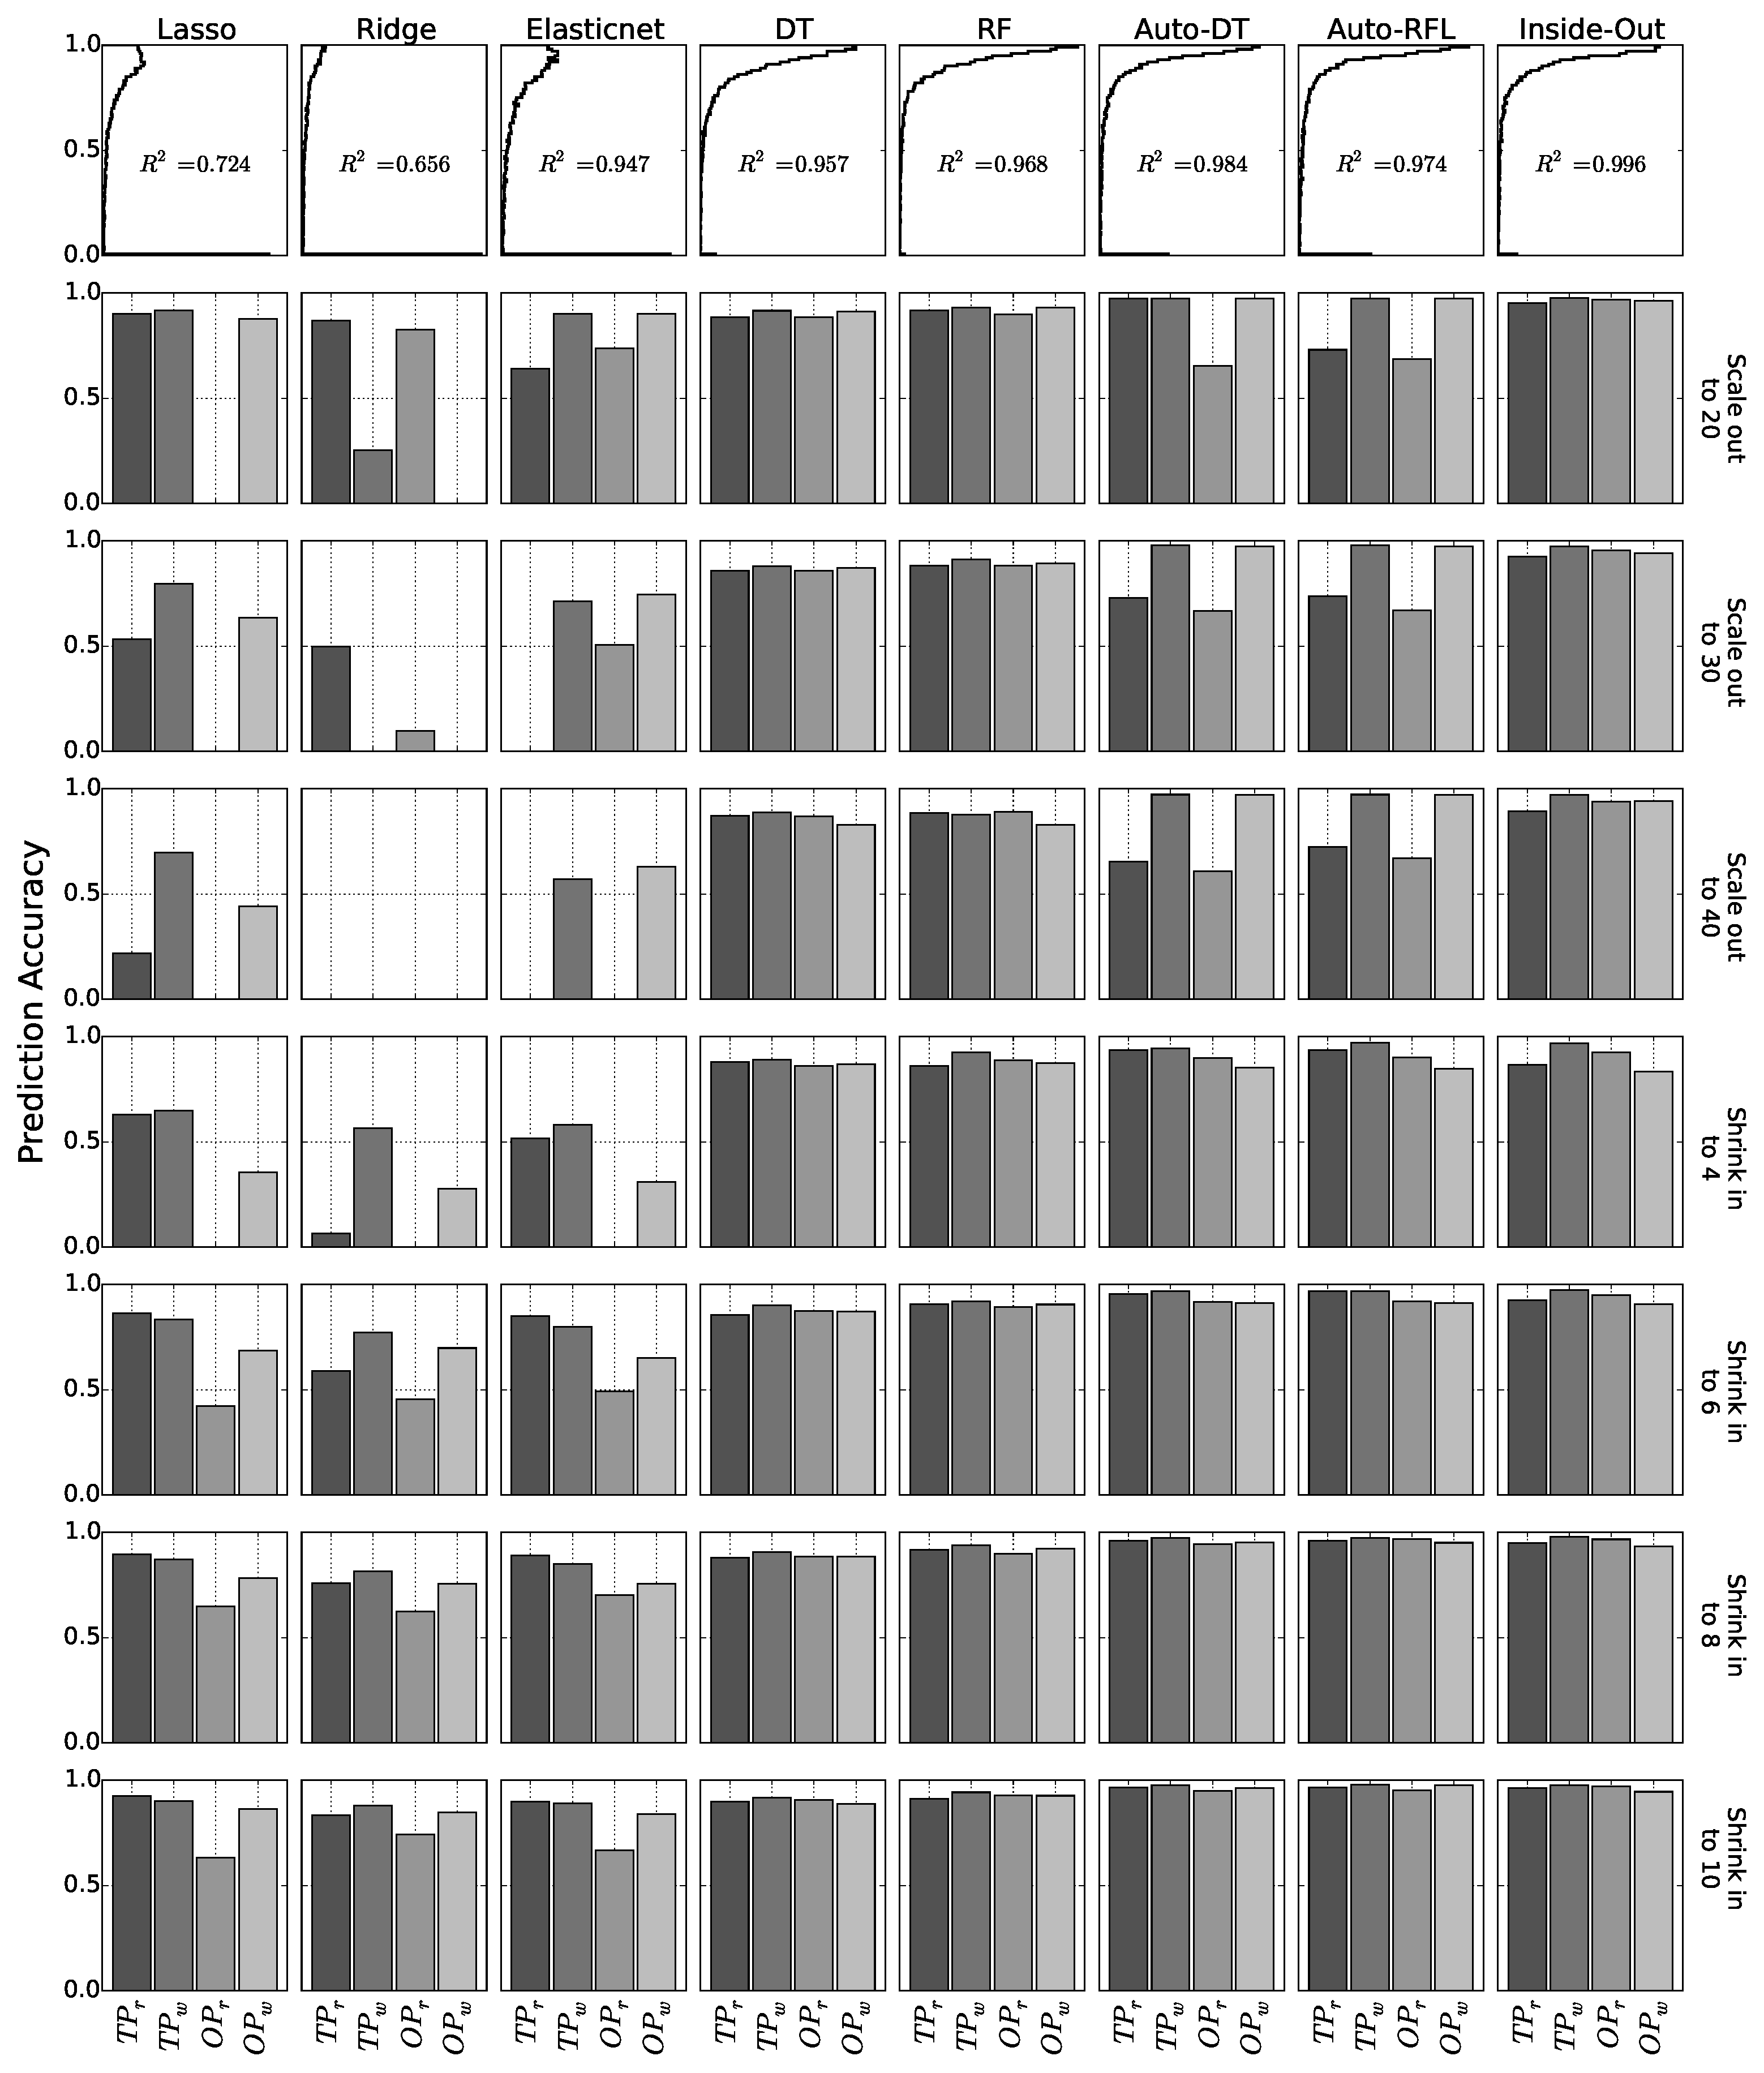
\includegraphics[width=0.9\textwidth]{Chapter-InsideOut/figures/unseen_scale_all_new.eps}
    \caption{Comparison of model performance in the on-demand scaling scenario. In the scale-out scenario, a performance model trained with 10 Ceph nodes is used to predict the performance of Ceph cluster with 20, 30 and 40 nodes.}
    \label{fig:elasticity}
\end{figure}


\subsection{Prediction Performance in a Multi-tenant Cloud}

This section examines the modeling performance of Inside-Out.
We first evaluate whether Inside-Out is able to extrapolate
performance of a larger Ceph cluster. 
Next, we evaluate how Inside-Out performs
when systems are subject to performance interference.

\subsubsection{Elastic Storage (On-demand Scaling)}
\label{sec:scaleout_prediction}

A storage service needs to grow or shrink its capacity on demand.
We evaluate Inside-Out's ability to capture the storage behavior at different system scales.
As shown in \myfigure{\ref{fig:elasticity}}, we use training data collected from 
4, 6, 8, and 10 nodes, and then predict the performance of 20, 30, and 40 nodes.
We also evaluate prediction accuracy in the \emph{shrink-in} scenario.
For both read and write throughput predictions, the linear models exhibit high variance.
In the $OP_r$ and $OP_w$ cases, the prediction results are not even comparable to the other methods.
Inside-Out, on the other hand, helps mitigate this issue, and achieves more than 90\% accuracy.
With increasing sizes of the storage, the prediction accuracy decreases because the prediction target 
becomes increasingly different from the training data.
Running a benchmark test against a very large system is time-consuming.
Here we demonstrate that Inside-Out can predict performance for systems that are 
four times larger than the system for which training data was collected.
%Due to resource limitations, we cannot show the upper bound of the largest system size that we can predict.
%However, we believe the upper bound can increase as the performance model keeps learning the system behavior.

\begin{figure}
    \centering
    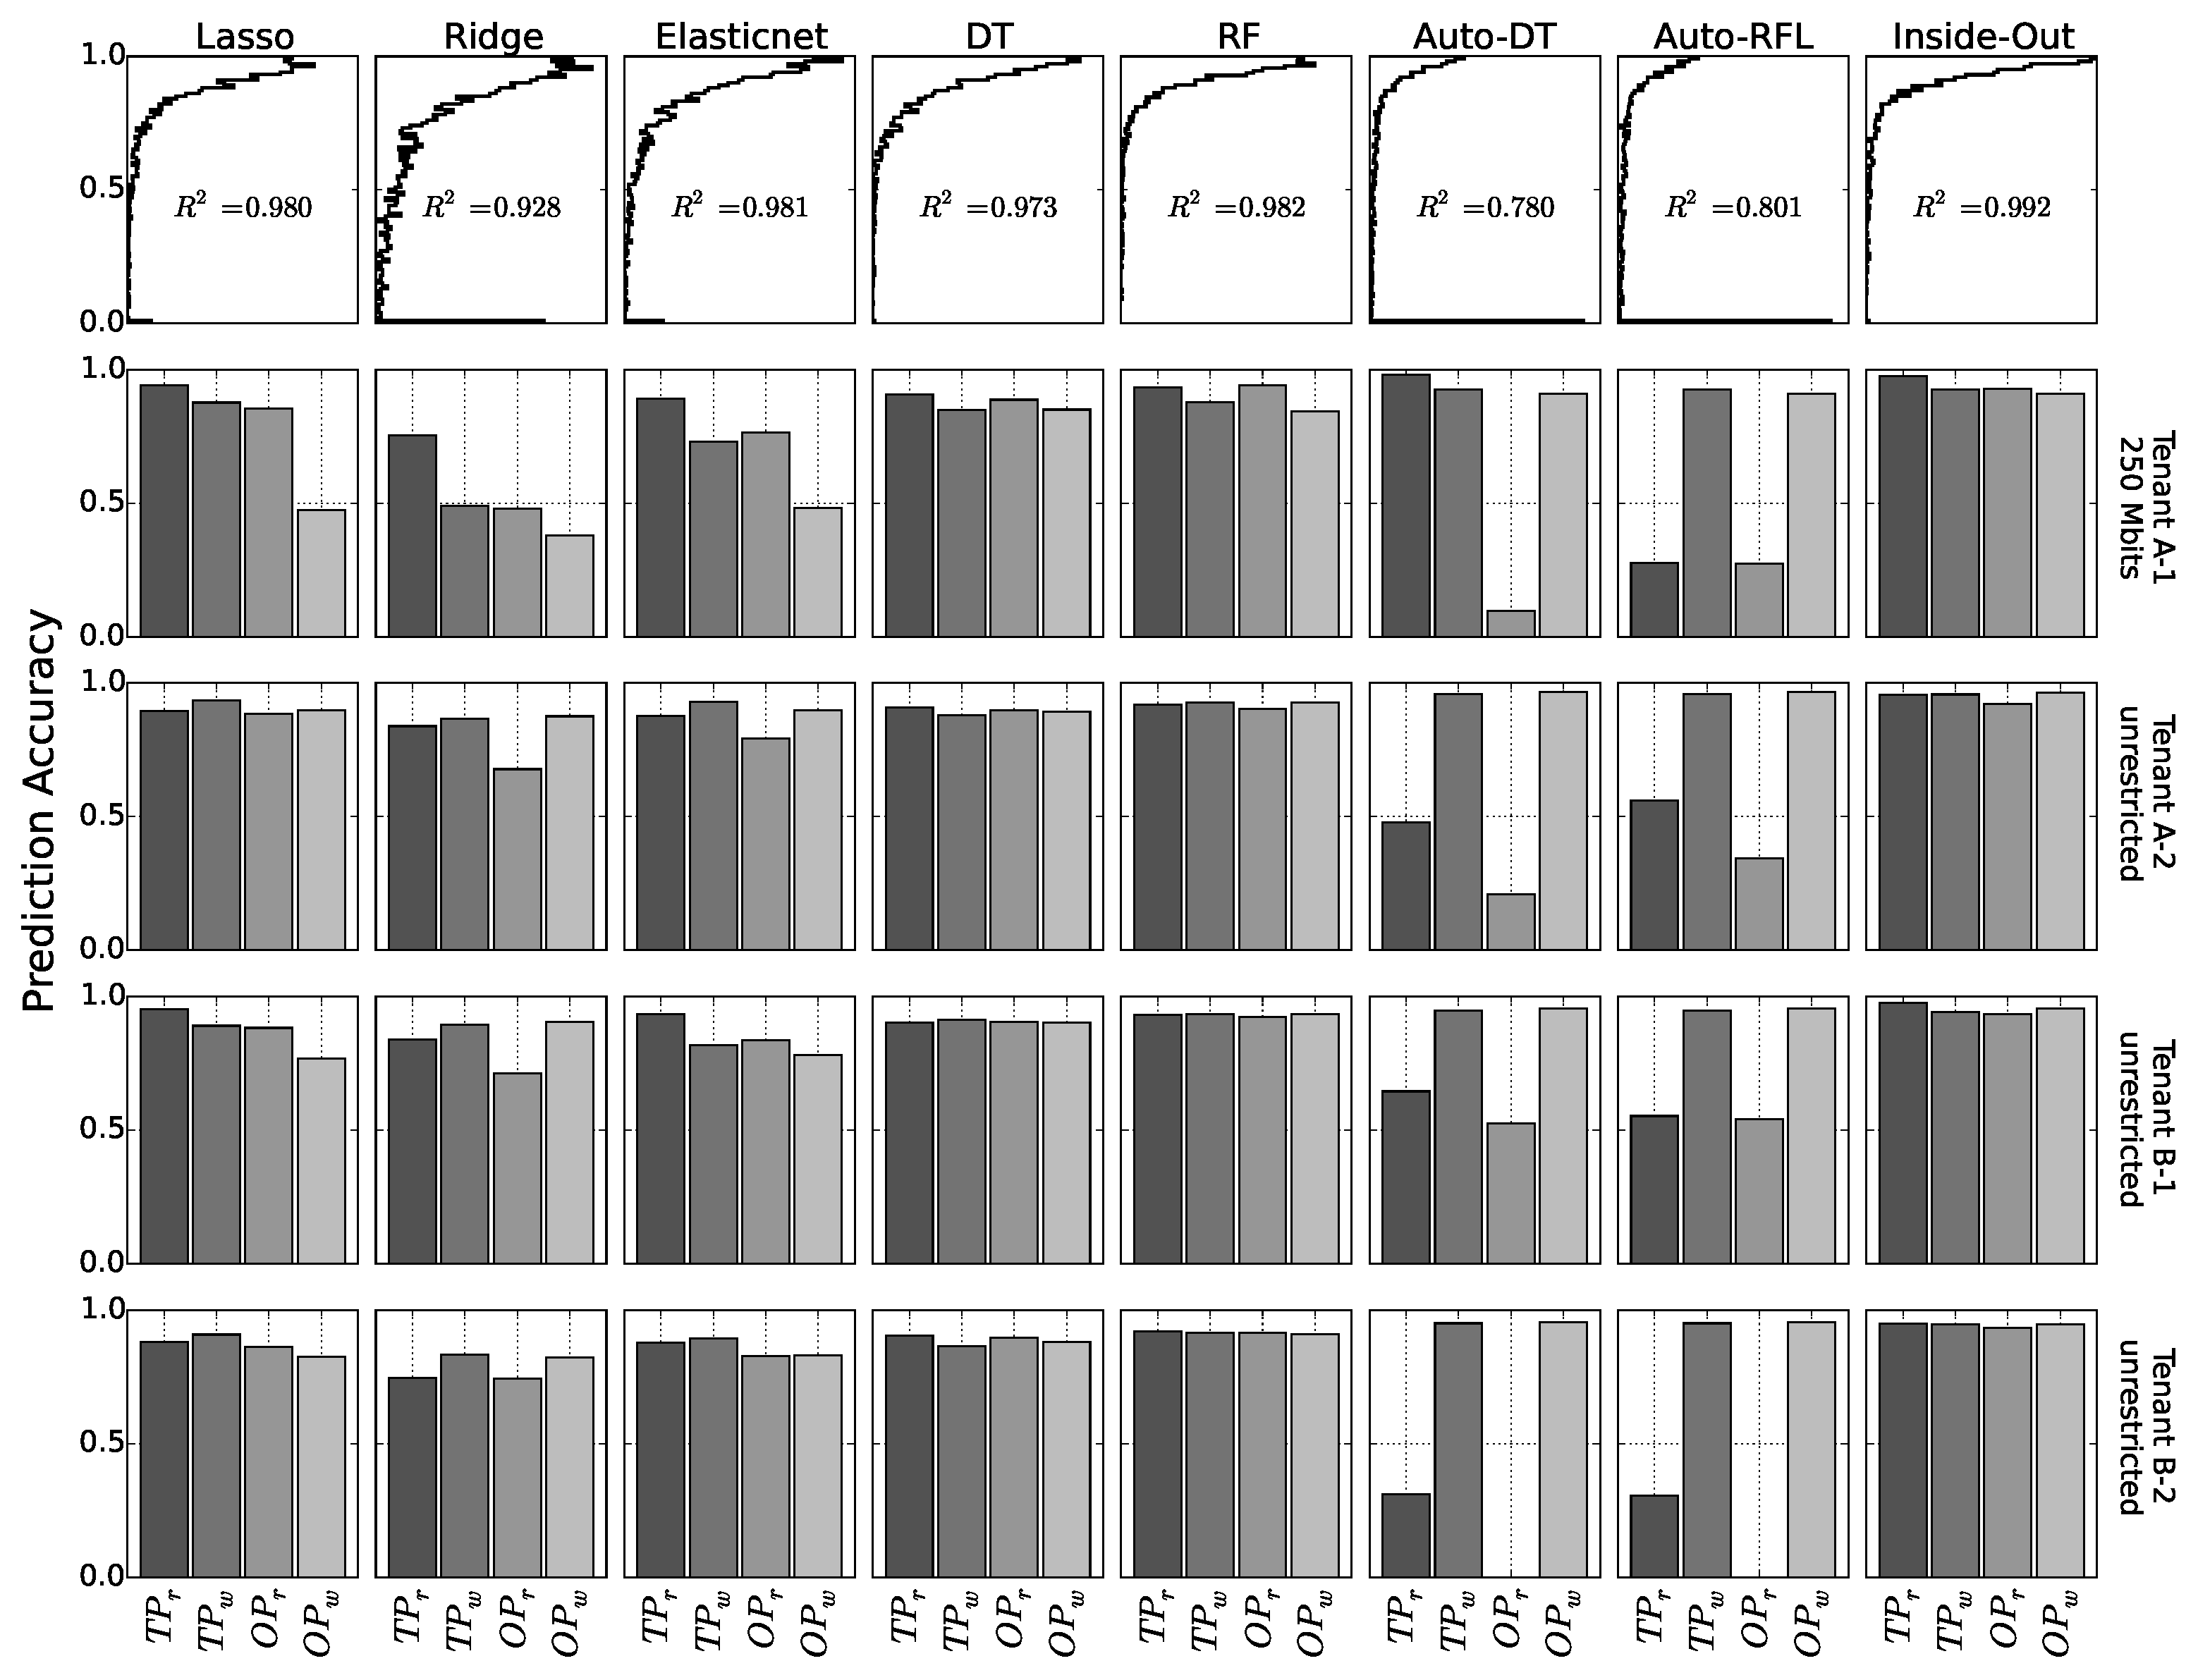
\includegraphics[width=0.9\textwidth]{Chapter-InsideOut/figures/multi_tenancy_all_new.eps}
    \caption{Prediction accuracy in a multi-tenancy scenario. Tenant A-1 is co-located with Tenant B-2. Tenant A-1 is throttled at 250Mbps. Tenant B-1 and B-2 are co-located without any traffic throttling.}
    \label{fig:multi_tenancy}
\end{figure}


\begin{figure*}
    \centering
    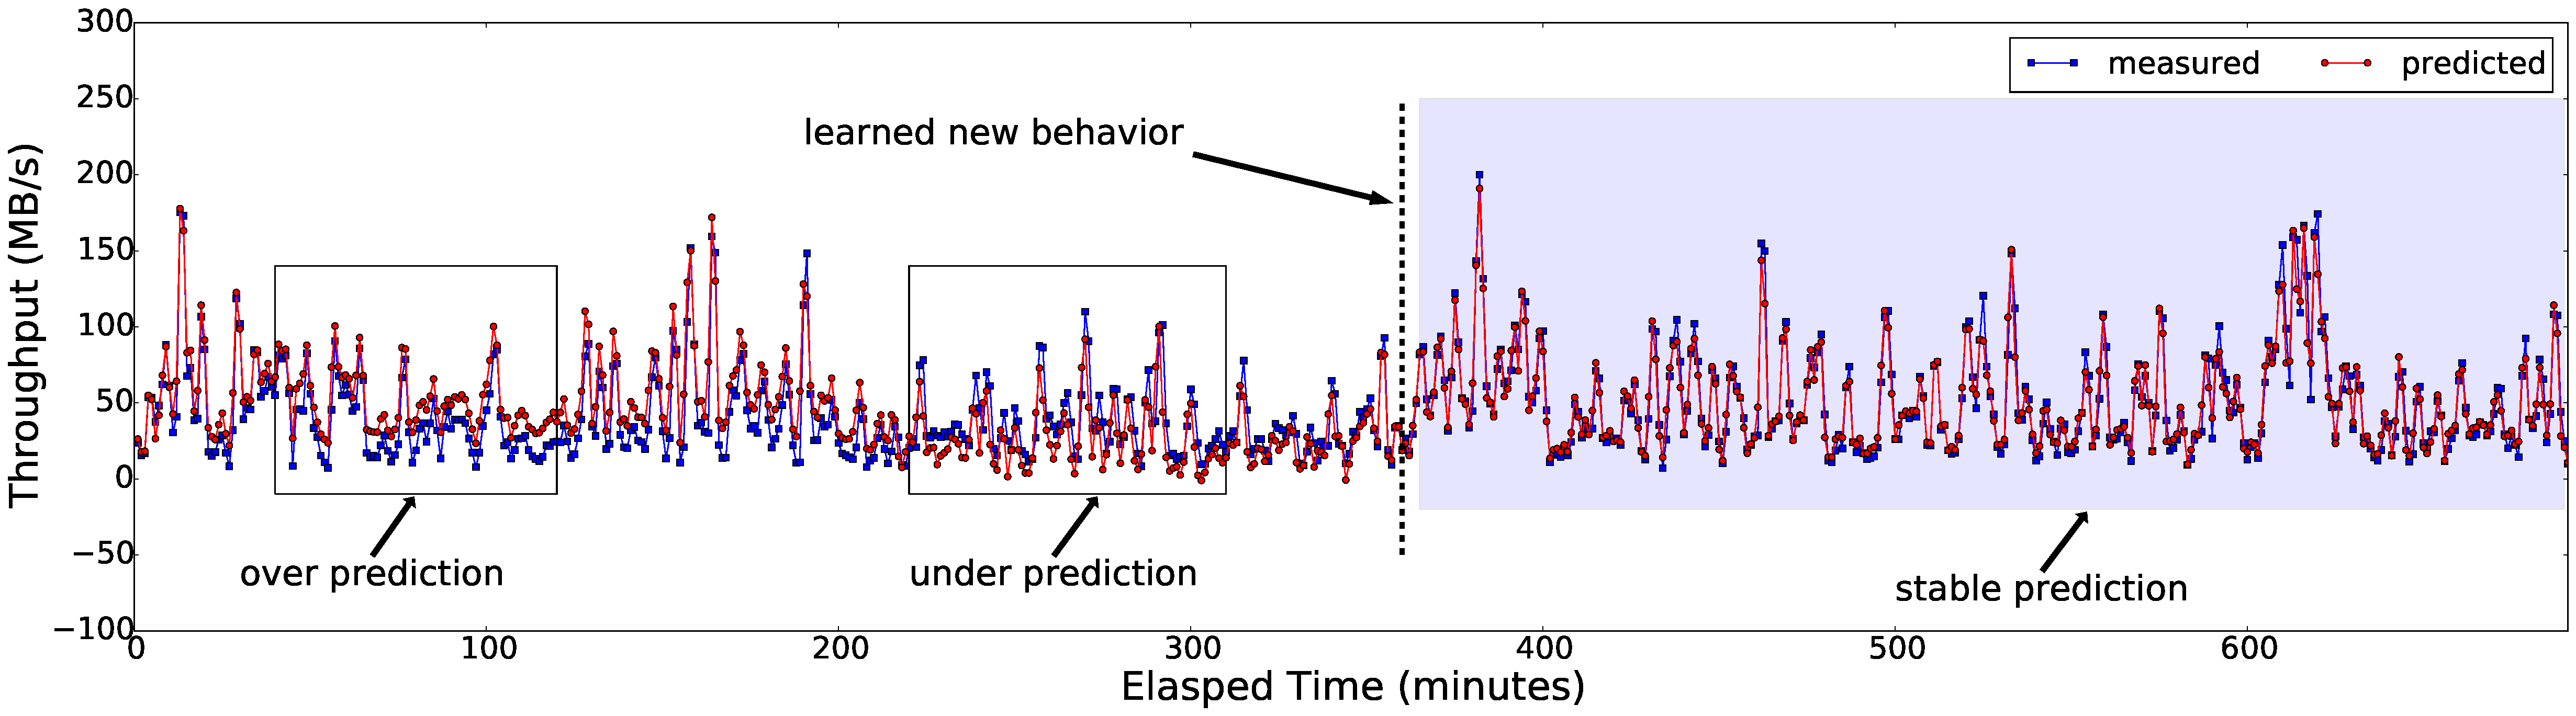
\includegraphics[width=0.9\textwidth]{Chapter-InsideOut/figures/real-world_tp_read.pdf}
    \caption{Application of Inside-Out to real time prediction of read throughput on a 10-node Ceph cluster.  Inside-Out starts from a simple prediction model trained by our collected benchmarking data.  Inside-Out keeps learning the storage behavior while improving prediction accuracy over time.}
    \label{fig:real_workload}
\end{figure*}


\subsubsection{Multi-Tenancy}
 
Next we evaluate Inside-Out's ability to adapt to performance interference among storage tenants.
We consider two cases for this evaluation. 
Each tenant runs a Ceph cluster with 10 OSDs separately, but tenants share the same 10 physical machines.
In the first case, we restrict the bandwidth of only the first tenant at 250Mbps.
%Two tenants compete for resources and \chin{\textbf{Tenant A-1}} has lower bandwidth SLO.
In the second case, we run two concurrent Ceph clusters but without network throttling.
\myfigure{\ref{fig:multi_tenancy}} shows that most prediction models are able to achieve more than 80\% accuracy.
The linear models like Ridge and Elasticnet yield lower prediction accuracies in some cases; however, Inside-Out performs well consistently.
Performance interference is challenging for a performance model designed for an isolated environment.
This evaluation demonstrates that the low-level performance metrics are good proxies for measuring
the end-to-end storage performance, even in a shared SDS environment.
%These metrics are able to reflect the behavior changes in the storage system.

%low-level performance feature selection approach is effective in capturing end-to-end performance, even under high storage interference.
%This property is important to SDS because it can help guarantee reliable end-to-end performance in a shared SDS environment.



\begin{comment}
\begin{figure*}
    \centering
    \includegraphics[width=0.9\textwidth]{figures/synthetic.eps}
    \caption{An online prediction scenario about six-hour long workload.  This synthetic workload is composed of 360 stages and each stage uniformly selects parameters such as workload types, request sizes and the number of clients.  The average stage duration is 60 seconds with standard deviation 20 seconds.}
\end{figure*}
\end{comment}

\begin{comment}
\begin{figure*}
    \centering
    \begin{subfigure}[b]{0.45\textwidth}
        \includegraphics[width=\textwidth]{figures/synthetic_read.eps}
        \caption{Read Throughput}
        \label{fig:synthetic_read}
    \end{subfigure}
    ~ %add desired spacing between images, e. g. ~, \quad, \qquad, \hfill etc.
      %(or a blank line to force the subfigure onto a new line)
    \begin{subfigure}[b]{0.45\textwidth}
        \includegraphics[width=\textwidth]{figures/synthetic_write.eps}
        \caption{Write Throughput}
        \label{fig:synthetic_write}
    \end{subfigure}
    \caption{An online prediction scenario about six-hour long workload.  This synthetic workload is composed of 360 stages and each stage uniformly selects parameters such as workload types, request sizes and the number of clients.  The average stage duration is 60 seconds with standard deviation 20 seconds.}
    \label{fig:synthetic_workload}
\end{figure*}
\end{comment}

%\subsection{Synthetic Workload}
\subsection{Online Self-Learning}
\label{sec:online_learning}

%Our goal is to apply Inside-Out to an online system so that SDS providers can guarantee the performance of a storage service hosted on their SDS platform.
%To evaluate this potential, 
Next, we create several synthetic workloads with mixed read/write ratios.
This synthetic workload spans 12 hours with 720 stages.
Each stage is 60-second long on average, with a standard deviation of 20 seconds.
We run four COSBench virtual machines for benchmarking and up to eight threads per COSBench client, with 10 Ceph OSDs and one monitor daemon.
We use Inside-Out to build an initial performance model with the training dataset described in Section~\ref{sec:dataset}.
\myfigure{\ref{fig:real_workload}} shows the prediction result for read throughput.
We can observe that the generated model can capture the overall trend, but suffers from over and under predictions.
This is because our training dataset is generated from a relatively clean environment, \ie the OS memory is flushed before any benchmarking process.
However, in the online prediction setting, cache is continuously consumed by non-stop client requests, which 
causes the real time storage behavior to be different from the training dataset.
With continuous monitoring of the performance of the storage service, 
we use Inside-Out to generate a new performance model at the sixth hour.
\myfigure{\ref{fig:real_workload}} shows that Inside-Out learns the new storage behavior and therefore, 
the over- and under-prediction issues are greatly mitigated.
%This evaluation demonstrates the potential of Inside-Out when applying it in an online system.
By continuously learning the storage behavior, SDS can accurately capture performance changes and therefore is able to provide reliable storage service.

%the problems due to over- and under-predictions are greatly mitigated.
%This evaluation demonstrates how Inside-Out can be used to continuously learn the storage behavior in an online system.


\begin{figure}
\centering
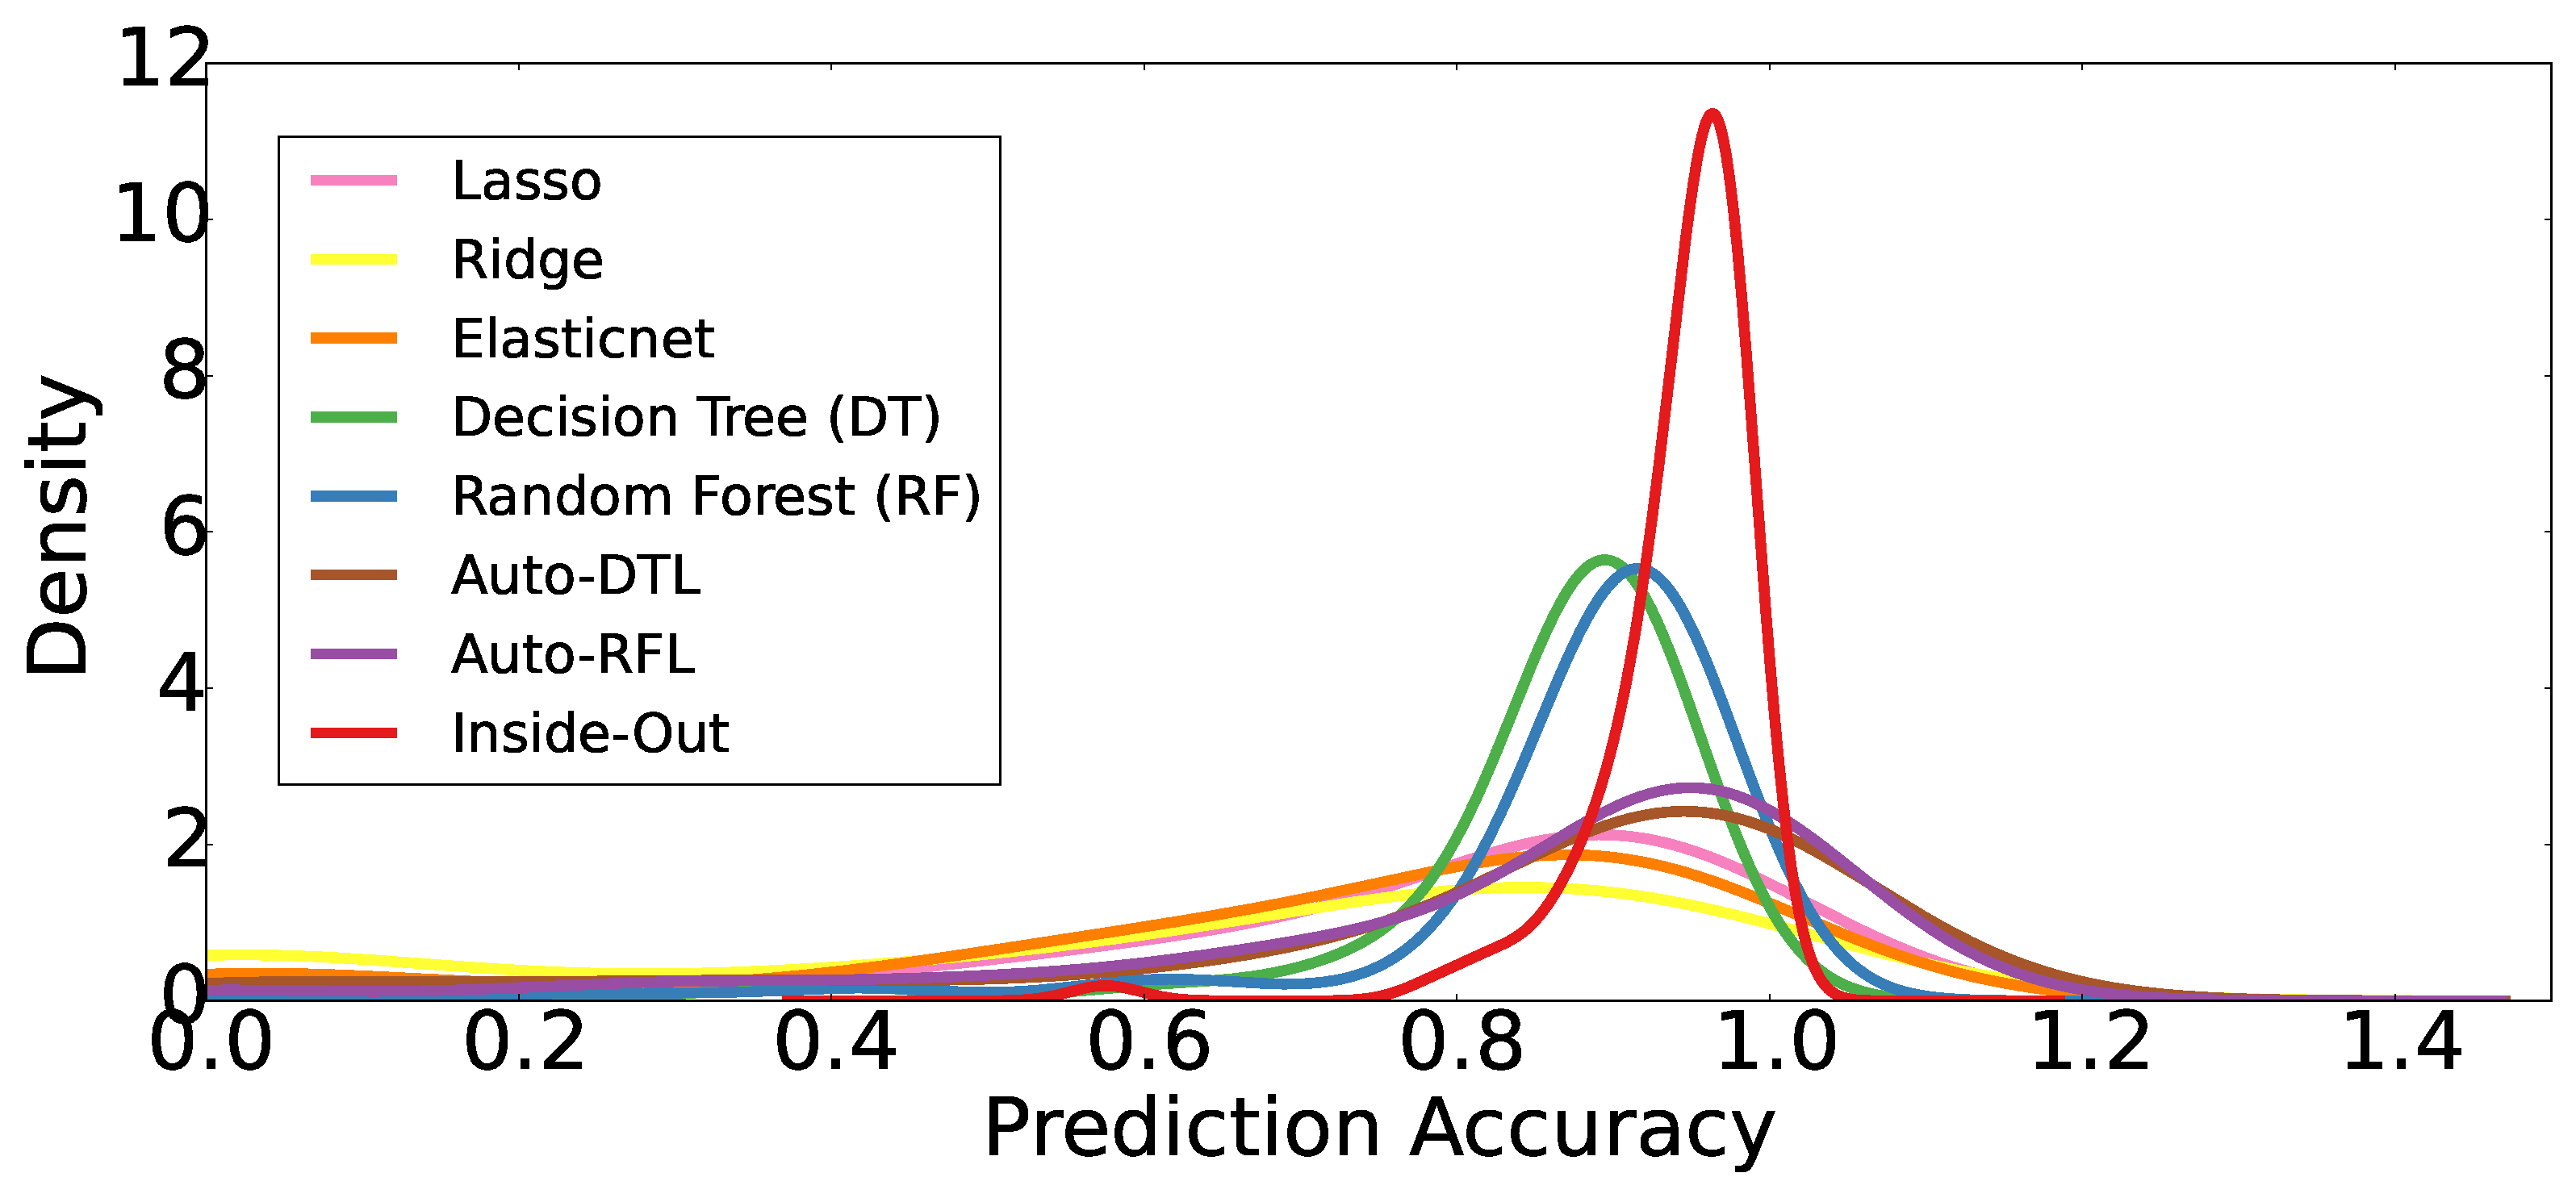
\includegraphics[width=0.9\textwidth, keepaspectratio]{Chapter-InsideOut/figures/aggregate_median.eps}
\caption{Kernel density function of prediction accuracy from \myfigure{\ref{fig:changing_workload}} to \myfigure{\ref{fig:multi_tenancy}}.  Each colored line represents the density function of a modeling approach.  Inside-Out is more consistent and accurate across almost every prediction case.}
\label{fig:aggregate}
\end{figure}


\vspace{1ex}
\subsection{Discussion}
We have shown that low-level performance metrics are useful to predict end-to-end throughput and IOPS.
%We applied Inside-Out to latency prediction and observe large variance and inconsistency.
%\chin{One} possible explanation is insufficient features and high variance in latency.
%The \chin{collected} low-level metrics are related to utilization, and these metrics might not provide enough information to fit a good model for predicting latency.
%Common approaches usually require request-level information \cite{Wang2004}.
%We need to further investigate latency prediction with other alternative generic low-level performance metrics.
Our evaluation has shown that low-level performance metrics are good indicators of end-to-end throughput and IOPS. 
Most existing performance models exhibit an inconsistent prediction behavior in the presence of diverse storage scenarios, 
such as changing workload, storage reconfigurations,
growing/shrinking storage, and multi-tenancy environments.
Our proposed two-level learning method can greatly improve prediction accuracy and yield consistent behavior.
Machine learning provides powerful tools, but they need to be used intelligently to achieve the best prediction accuracy. 
\myfigure{\ref{fig:aggregate}} shows the kernel density function of prediction accuracy across all prediction scenarios.
Inside-Out is a clear winner in terms of accuracy and consistency. 
More importantly, Inside-Out is able to learn new storage behavior, thereby enabling the performance model to adapt to the complex SDS environment.




